\documentclass[12pt]{article}

\usepackage{sbc-template}
\usepackage{graphicx,url}
\usepackage[utf8]{inputenc}
\usepackage[brazil]{babel}
\usepackage{float}
     
\sloppy

\title{Aquitetura de Computadores --- DGEMM}

\author{Matheus da Silva Conceição --- DRE\: 125050534}

\address{PESC --- Universidade Federal do Rio de Janeiro (UFRJ)
  \email{matheuswnscf@poli.ufrj.br}
}

\begin{document} 

\maketitle

\section{Introdução}
O objetivo deste trabalho é implementar algoritmos de multiplicação de matrizes 
para demonstrar as ideias do livro \textit{Computer Organization and Design: RISCV} de Hennessy e Patterson.
A cada capítulo do livro, um algoritmo de multiplicação de matrizes é implementado e cada um desses algoritmos
possui uma otimização específica.

\section{Algoritmo 1: Multiplicação de matrizes tradicional}
\subsection{Python puro}
O algoritmo tradicional de multiplicação de matrizes é o mais simples e direto, 
onde cada elemento da matriz resultante é calculado como a soma dos produtos 
dos elementos correspondentes das linhas da primeira matriz e das colunas da segunda matriz. 
A implementação em Python puro pode ser feita utilizando três 
loops aninhados para iterar sobre as linhas e colunas das matrizes.

\begin{figure}[H]
    \centering
    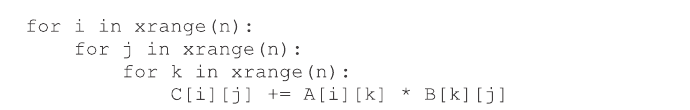
\includegraphics[width=0.8\textwidth]{images/1.png} 
    \caption{Implementação do algoritmo em Python.}\label{fig:fig1}
\end{figure}

Como é um dos mais simples, o algoritmo tradicional tem uma complexidade de tempo de O (n$^3$),
 o que o torna ineficiente para matrizes grandes. Além disso, para esse algoritmo, em mais baixos níveis,
 para executar cada multiplicação, o processador precisa acessar a memória para obter os valores das matrizes
 inúmeras vezes. Outra questão também é o que os dados do Python puro (como o Float) contam com
 objetos, isso somado a fato das listas serem estruturas de dados mais complexas (listas dentro de listas), torna o processo 
 de multiplicação ainda mais lento.

 \subsection{Numpy (biblioteca do Python)}
 Já o algoritmo de multiplicação de matrizes utilizando a biblioteca Numpy (uma biblioteca com foco
em computação numérica e álgebra linear) é muito mais rápido e eficiente.
A biblioteca Numpy é otimizada para operações de matrizes e utiliza implementações em C (como listas contíguas),
o que deixa a multiplicação de matrizes muito mais rápida do que a implementação em Python puro.

\section{Algoritmo 2: Multiplicação de matrizes utilizando C}

A implementação do algoritmo de multiplicação de matrizes utilizando a linguagem C é significativamente 
mais rápida do que a implementação em Python puro. Primeiramente, diferentemente do Python puro, \textbf{em C os dados
das matrizes são armazenados em arrays contíguos na memória}, ou seja, os dados na memória estão organizados de forma
sequencial, o que permite um acesso mais eficiente à memória. Além disso, a linguagem C é compilada, 
o que significa que o código é traduzido diretamente para código de máquina, eliminando a etapa de 
interpretação presente no Python. Isso resulta em uma execução mais rápida, 
especialmente para operações intensivas em cálculos, como a multiplicação de matrizes.

\begin{figure}[H]
    \centering
    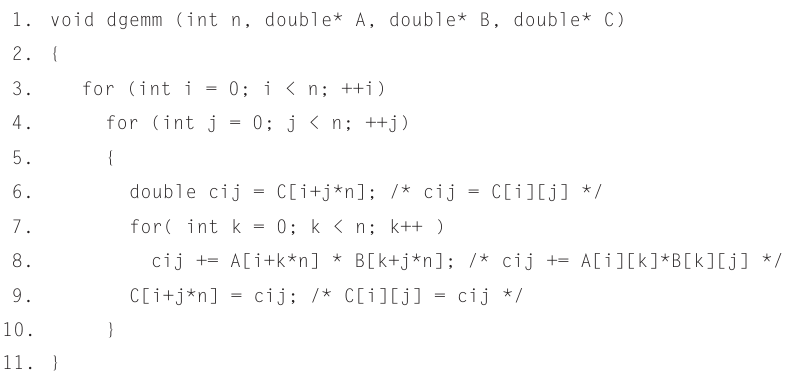
\includegraphics[width=0.8\textwidth]{images/2.png} 
    \caption{Implementação do algoritmo em C.}\label{fig:fig2}
\end{figure}

\section{Algoritmo 3: otimização AVX}

A otimização AVX (Advanced Vector Extensions) é uma extensão do conjunto de instruções x86 que
permite a execução de operações vetoriais em paralelo, isso através de um conceito chamado SIMD 
(Single Instruction, Multiple Data) ou ``subword parallelism'', definição que o livro texto utiliza.

Em vez de processar um elemento de cada vez, a otimização AVX permite que o processador 
execute a mesma operação em vários elementos simultaneamente, utilizando registradores vetoriais de 256 ou 512 
bits.

\begin{figure}[H]
    \centering
    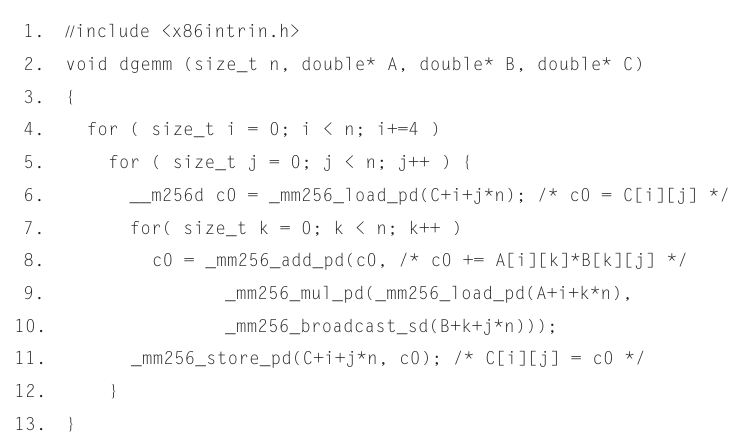
\includegraphics[width=0.8\textwidth]{images/3.png} 
    \caption{Implementação da otimização AVX.}\label{fig:fig3}
\end{figure}

Primeiramente, a declaração \texttt{\_m256d} é um tipo de dado específico para armazenar vetores de 256 bits, 
que podem conter quatro números de ponto flutuante de precisão dupla (double). A função 
\texttt{\_mm256\_loadu\_pd} é usada para carregar os dados consecutivos (por exemplo, 4 elementos de uma única linha ou 
coluna) das matrizes A e B para os registradores vetoriais, permitindo que as operações sejam 
realizadas em paralelo. A função \texttt{\_mm256\_mul\_pd} multiplica 
os elementos correspondentes dos vetores, e a função \texttt{\_mm256\_add\_pd} é usada para acumular 
os resultados da multiplicação. Por fim, a função \texttt{\_mm256\_storeu\_pd} armazena o 
resultado final da multiplicação de matrizes de volta na matriz C.

O bom desempenho da otimização AVX se deve à capacidade de processar múltiplos 
elementos em paralelo, reduzindo o número de ciclos de clock necessários para 
realizar a multiplicação de matrizes. 


\section{Algoritmo 4: Otimização AVX com Loop Unrolling}

Avançando para uma implementação mais sofisticada, a otimização passa a combinar o Paralelismo no Nível de Dados (SIMD) com o Paralelismo no Nível de Instrução (ILP). O diferencial desta etapa é a aplicação da técnica de \textit{Loop Unrolling} (desenrolamento de laço) com um fator de 4. Em vez de utilizar apenas um vetor acumulador, é declarado um arranjo de registradores \texttt{\_\_m256d c[UNROLL]}. Isso expõe para o processador quatro operações matemáticas completamente independentes a cada iteração do laço.

\begin{figure}[H]
    \centering
    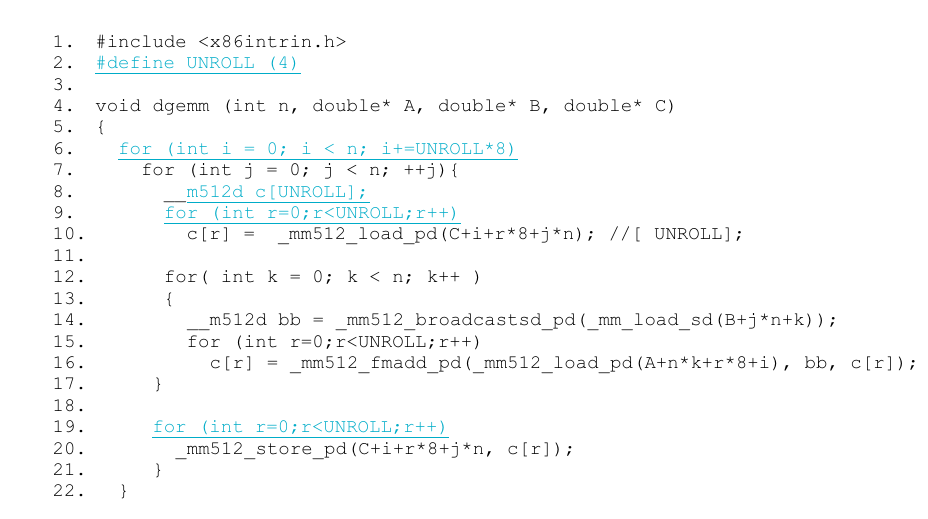
\includegraphics[width=0.8\textwidth]{images/4.png} 
    \caption{Implementação da otimização AVX com Loop Unrolling.}\label{fig:fig4}
\end{figure}

Para otimizar ainda mais o gargalo de acesso à memória, a instrução \texttt{\_mm256\_broadcast\_sd} é empregada para ler um único elemento escalar da matriz B e replicá-lo de forma imediata por todo um registrador vetorial. O compilador reaproveita esse mesmo registrador nas multiplicações subsequentes. A operação matemática central é feita através da instrução \texttt{\_mm256\_fmadd\_pd} (Fused Multiply-Add), que realiza a multiplicação dos vetores de A e B e o acúmulo em C em uma única instrução de hardware de alta velocidade.

O bom desempenho dessa abordagem ocorre porque o código fornece à arquitetura superescalar da CPU um fluxo contínuo de instruções. Graças à independência de dados nos registradores acumuladores e à capacidade de execução fora de ordem do processador, os cálculos ocorrem em paralelo contínuo, evitando bolhas de ociosidade (\textit{stalls}) no \textit{pipeline}.

\section{Algoritmo 5: Otimização com Cache Blocking}

O próximo passo na otimização da função DGEMM foca em transpor o gargalo da hierarquia de memória do processador, introduzindo a técnica de \textit{Cache Blocking}. Quando matrizes de grandes dimensões são multiplicadas utilizando a abordagem tradicional, o volume de dados excede rapidamente a capacidade das memórias cache de nível 1 (L1) e 2 (L2). Isso provoca uma alta taxa de \textit{cache misses}, forçando a CPU a buscar dados repetidamente na memória principal (RAM), penalizando o desempenho de forma severa.

Para mitigar esse problema, a implementação foi refatorada para iterar sobre a matriz em submatrizes quadradas menores, cujo tamanho é definido pela constante \texttt{BLOCKSIZE = 32}. Através de laços de repetição externos adicionais, o algoritmo particiona o problema, enquanto a função auxiliar \texttt{do\_block} concentra-se em resolver a multiplicação exclusivamente para aquele pequeno bloco. Como este subconjunto de dados de 32x32 elementos cabe inteiramente na cache L1, as operações matemáticas reutilizam os valores já carregados na memória de acesso ultrarrápido (maximizando o reuso temporal e espacial da cache).

\section{Especificações e métricas de teste}
\subsection{Especificações do ambiente de teste}
    \begin{itemize}
        \item Processador: Ryzen 7 5700X (8 núcleos, 16 threads, 3.8 GHz base, 4.6 GHz boost)
        \item Placa de vídeo: AMD Radeon RX 6750 XT
        \item Memória RAM:\@32 GB DDR4
        \item Sistema Operacional: Linux Ubuntu
        \item Compilador: GCC 13.3.0
        \item Python: 3.12.3
        \item SSD:\@1 TB NVMe
        \item Todos os testes foram realizados utilizando o mesmo ambiente para garantir a consistência dos resultados: PC em Idle e sem outros processos em execução.
    \end{itemize}

\subsection{Métricas de teste}
\begin{itemize}
    \item Tempo de execução: O tempo total gasto para multiplicar matrizes de diferentes tamanhos.
    \item Tamanho das matrizes: Matrizes quadradas de tamanhos 512$\times$512, 1024$\times$1024, 2048$\times$2048, 4096$\times$4096 e 8192$\times$8192.
    \item Testes repetidos: Cada teste foi executado 5 vezes para cada tamanho de matriz, e a média dos tempos de execução foi calculada para garantir a precisão dos resultados.
    \item Desvio padrão: O desvio padrão dos tempos de execução foi calculado para avaliar a variabilidade dos resultados.
    \item Máximo e mínimo: Os tempos máximo e mínimo de execução foram registrados para cada teste para identificar possíveis outliers.
    \item Comparação de desempenho: Os tempos de execução dos diferentes algoritmos foram comparados para avaliar o impacto das otimizações implementadas.
\end{itemize}

\section{Análise de resultados}

Os gráficos mostram a evolução das otimizações. Fica evidente que o Python puro é inadequado para computação intensiva, justificando a necessidade de linguagens de baixo nível. A versão em C sem otimizações (apenas compilada) já traz um ganho, mas é a combinação de SIMD (AVX), ILP (Loop Unrolling) e Localidade de Memória (Cache Blocking) que melhora de fato a performance.

\subsection*{Pontos de destaque}
\subsection{Gargalo de Memória}
O algoritmo tradicional (AVX + Loop Unrolling) sofre com o gargalo de memória, pois cada multiplicação exige múltiplos acessos à RAM, resultando em um grande número de \textit{cache misses}. A otimização com Cache Blocking reduz significativamente esse problema, mantendo os dados necessários na cache L1 e melhorando o desempenho. Isso fica evidente nos gráficos, onde para uma matriz pequena o algoritmo alcança um desempenho de 9.8 GFLOPS, mas para matrizes maiores o desempenho cai drasticamente.

\subsection{Numpy}
A biblioteca Numpy, apesar de ser escrita em Python, teve um desempenho bem satisfatório. Isso se deve ao fato de que a biblioteca é otimizada para operações de matrizes e utiliza implementações em C, o que permite um acesso mais eficiente à memória e uma execução mais rápida do que a implementação em Python puro, essas otimizações deram um ganho que permitiram ultrapassar a performance do algoritmo tradicional em C sem otimizações e até com otimização AVX.


\end{document}
